\documentclass[a4paper, 11pt]{article}
\usepackage{comment}
\usepackage{fullpage}
\usepackage{amsmath}
\usepackage{amssymb}
\usepackage{mathtools}
\usepackage{fontspec}
\defaultfontfeatures{Ligatures=TeX}
\usepackage{xfrac}
\usepackage{icomma}
\usepackage[section,below]{placeins}
\usepackage[labelfont=bf,font=small,width=0.9\textwidth]{caption}
\usepackage{subcaption}
\usepackage{graphicx}
\usepackage{grffile}
\usepackage{float}
\floatplacement{figure}{htbp}
\floatplacement{table}{htbp}
\usepackage{booktabs}
\usepackage{hyperref}
\usepackage[ngerman]{babel}
\usepackage{pdfpages}
\begin{document}
\noindent
%\centerline{\small{\textsc{Technische Universität Dortmund}}} \\
\large{\textbf{5. Übungsblatt zur Vorlesung \hfill WS 2017/2018 \\
Statistische Methoden der Datenanalyse \hfill Prof. W. Rhode}} \\
Annika Burkowitz, Sebastian Bange, Alexander Harnisch \\
\noindent\makebox[\linewidth]{\rule{\textwidth}{0.4pt}}

\section*{Aufgabe 16}
Die Zahlenwerte hängen von der genauen Gestalt der Populationen ab und werden von unserem Programm ausgegeben.

\subsection*{d)}
\begin{figure}
    \centering
    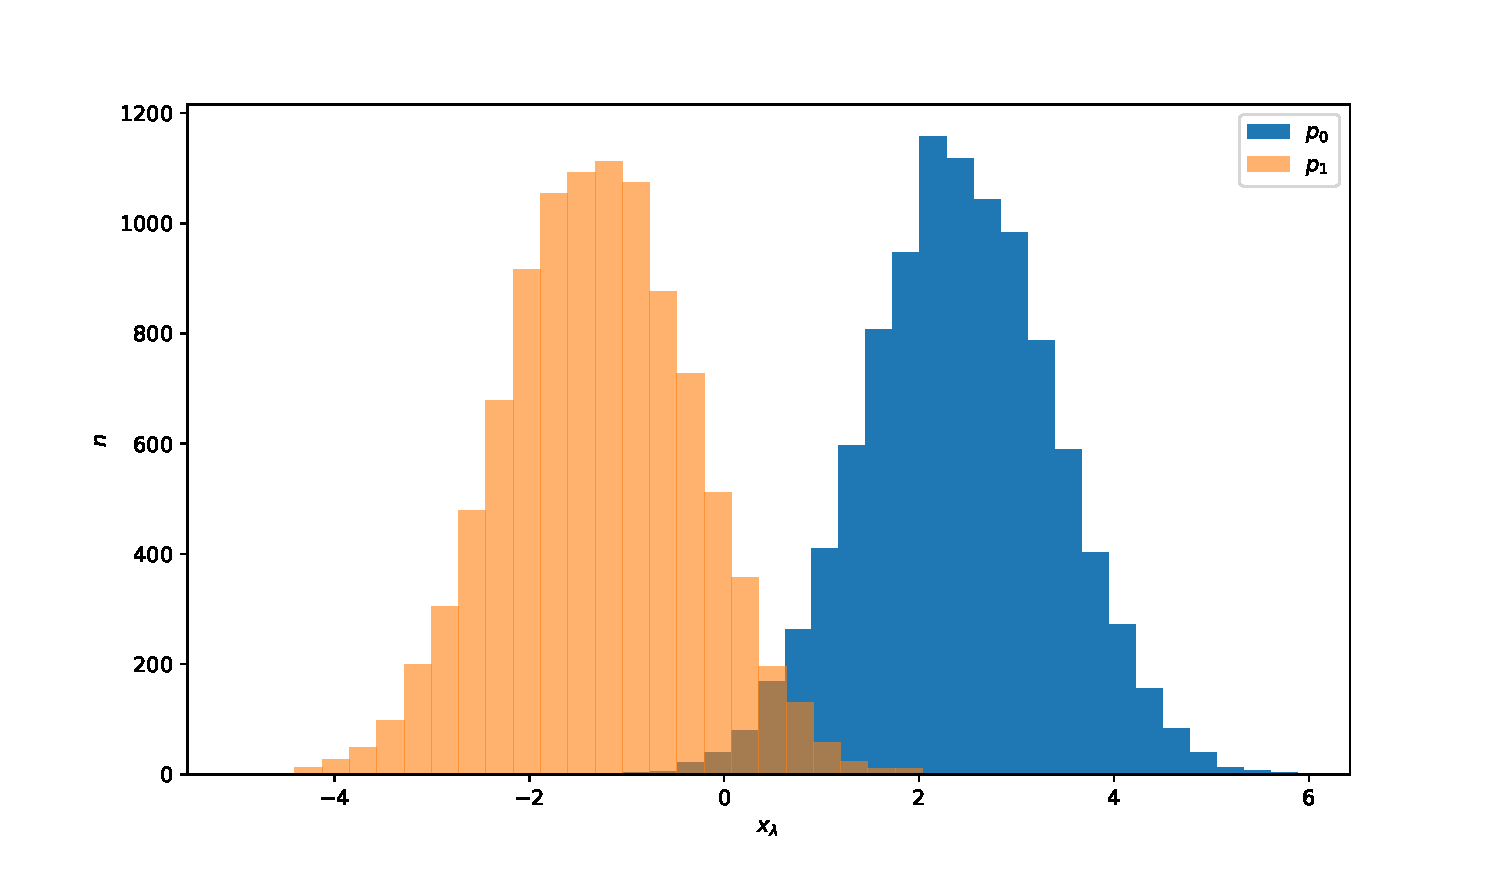
\includegraphics[width=\textwidth]{../A16/A16d_10000.pdf}
    \caption{Histogramm der Projektion für $P_{0, 10000}$.}
    \label{fig:A16d_10000}
\end{figure}
\begin{figure}
    \centering
    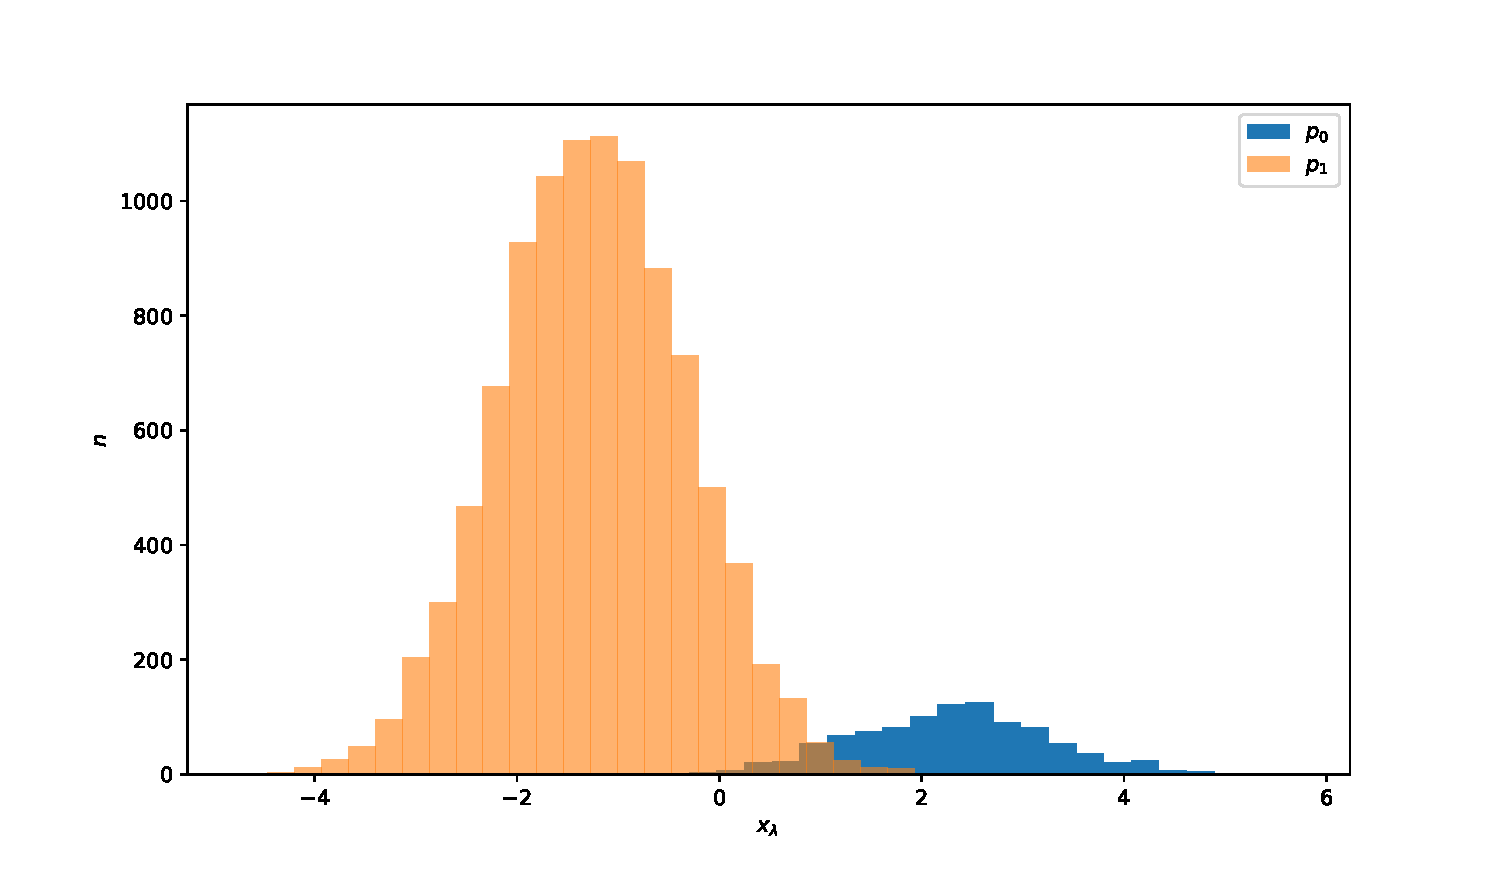
\includegraphics[width=\textwidth]{../A16/A16d_1000.pdf}
    \caption{Histogramm der Projektion für $P_{0, 1000}$.}
    \label{fig:A16d_1000}
\end{figure}
\FloatBarrier

\subsection*{e)}
\begin{figure}
    \centering
    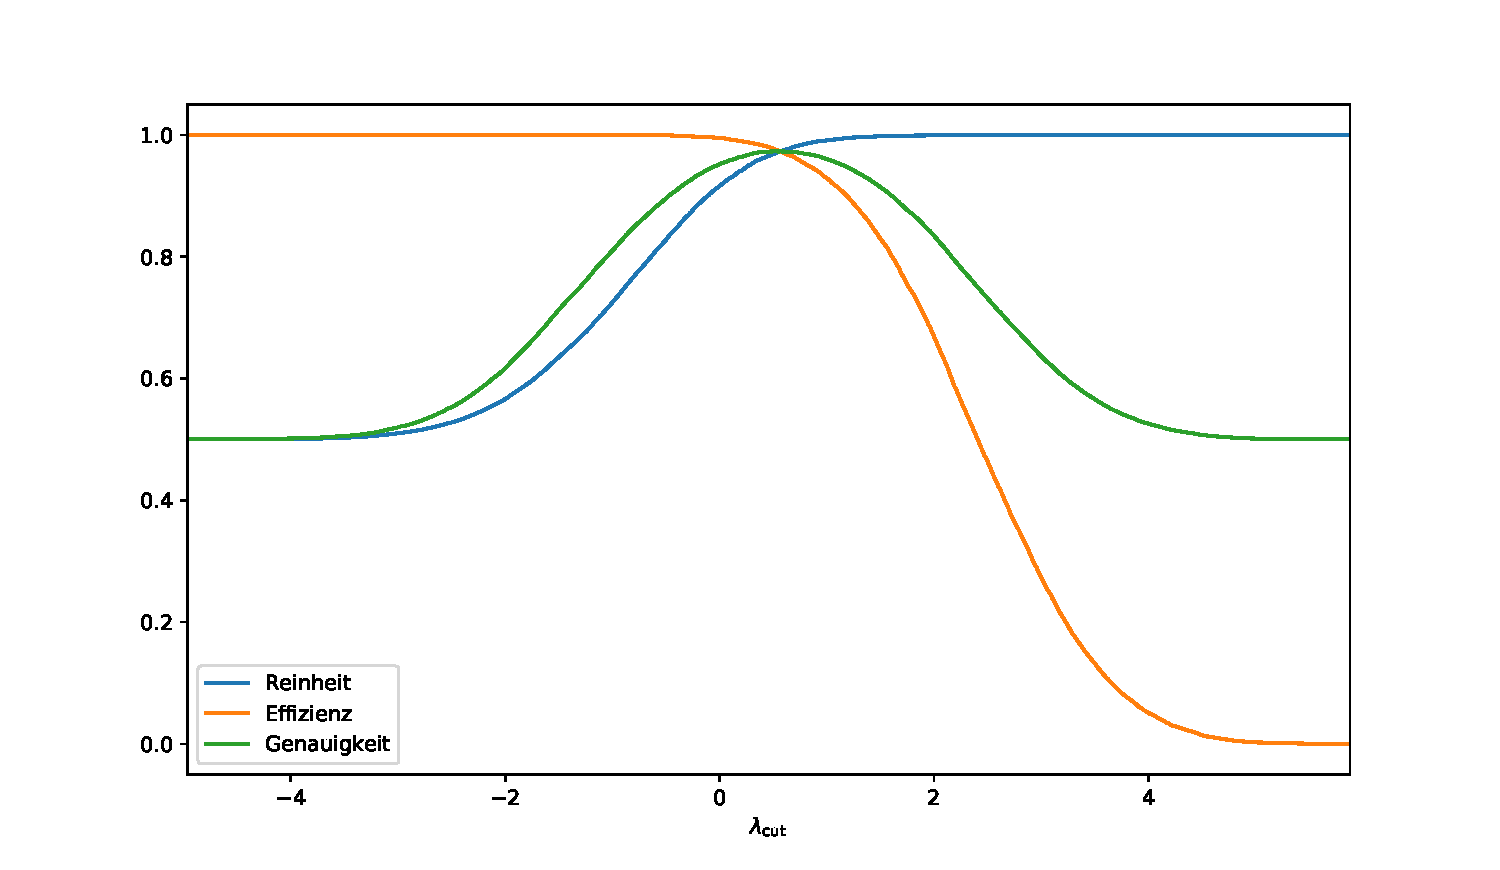
\includegraphics[width=\textwidth]{../A16/A16e_10000.pdf}
    \caption{Effizienz, Reinheit und Genauigkeit für $P_{0, 10000}$.}
    \label{fig:A16e_10000}
\end{figure}
\begin{figure}
    \centering
    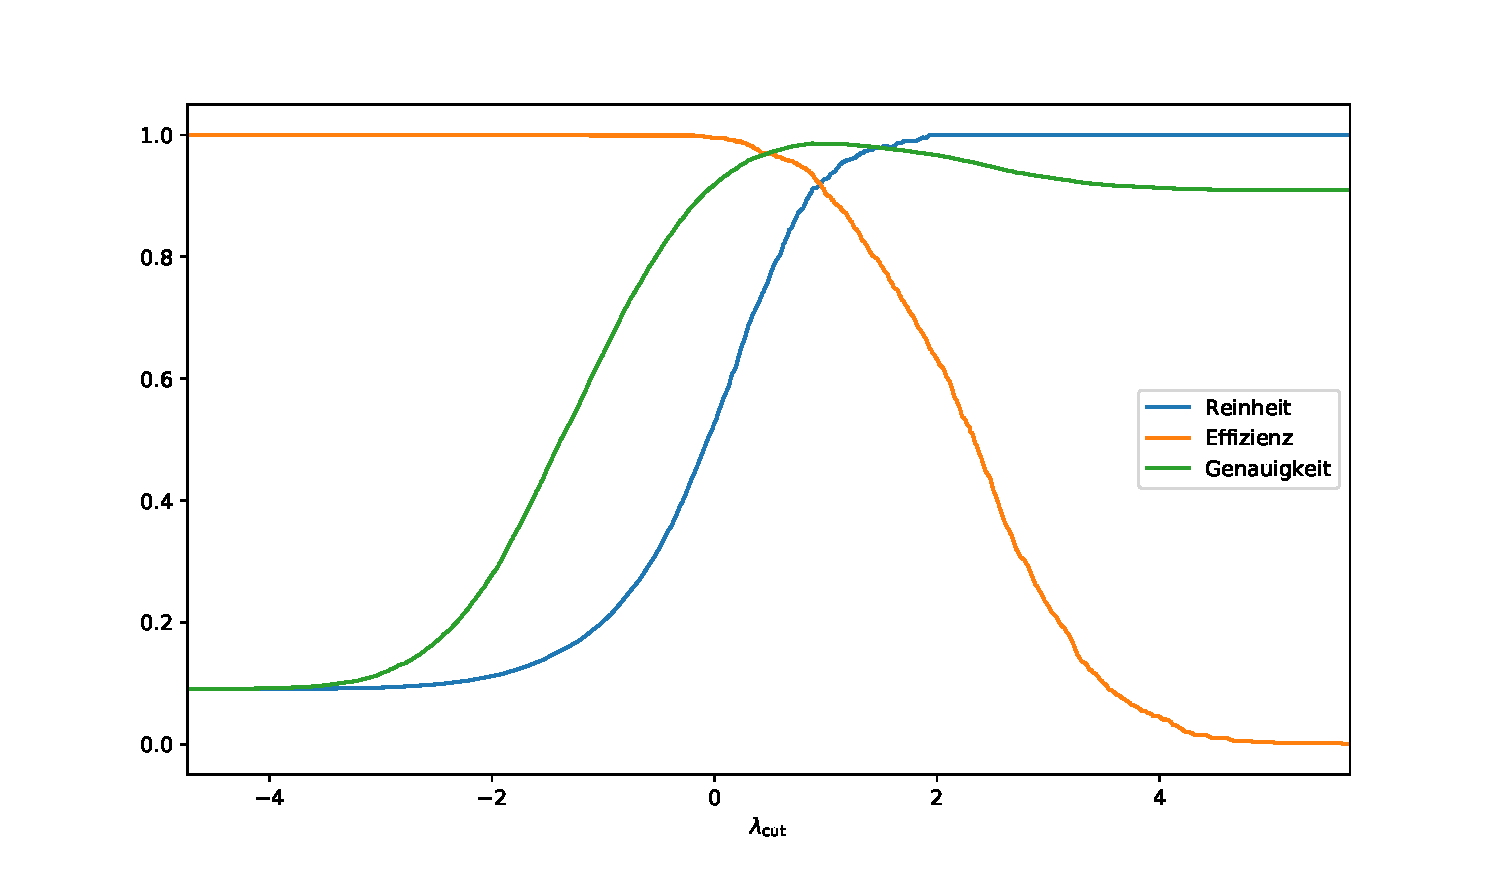
\includegraphics[width=\textwidth]{../A16/A16e_1000.pdf}
    \caption{Effizienz, Reinheit und Genauigkeit für $P_{0, 1000}$.}
    \label{fig:A16e_1000}
\end{figure}
\FloatBarrier

\subsection*{f)}
Das Signal-zu-Untergrundverhältnis $\frac{S}{B}$ wird maximal für $B \rightarrow 0$ also für $\lambda_\textup{cut} \rightarrow -\infty$.
\begin{figure}
    \centering
    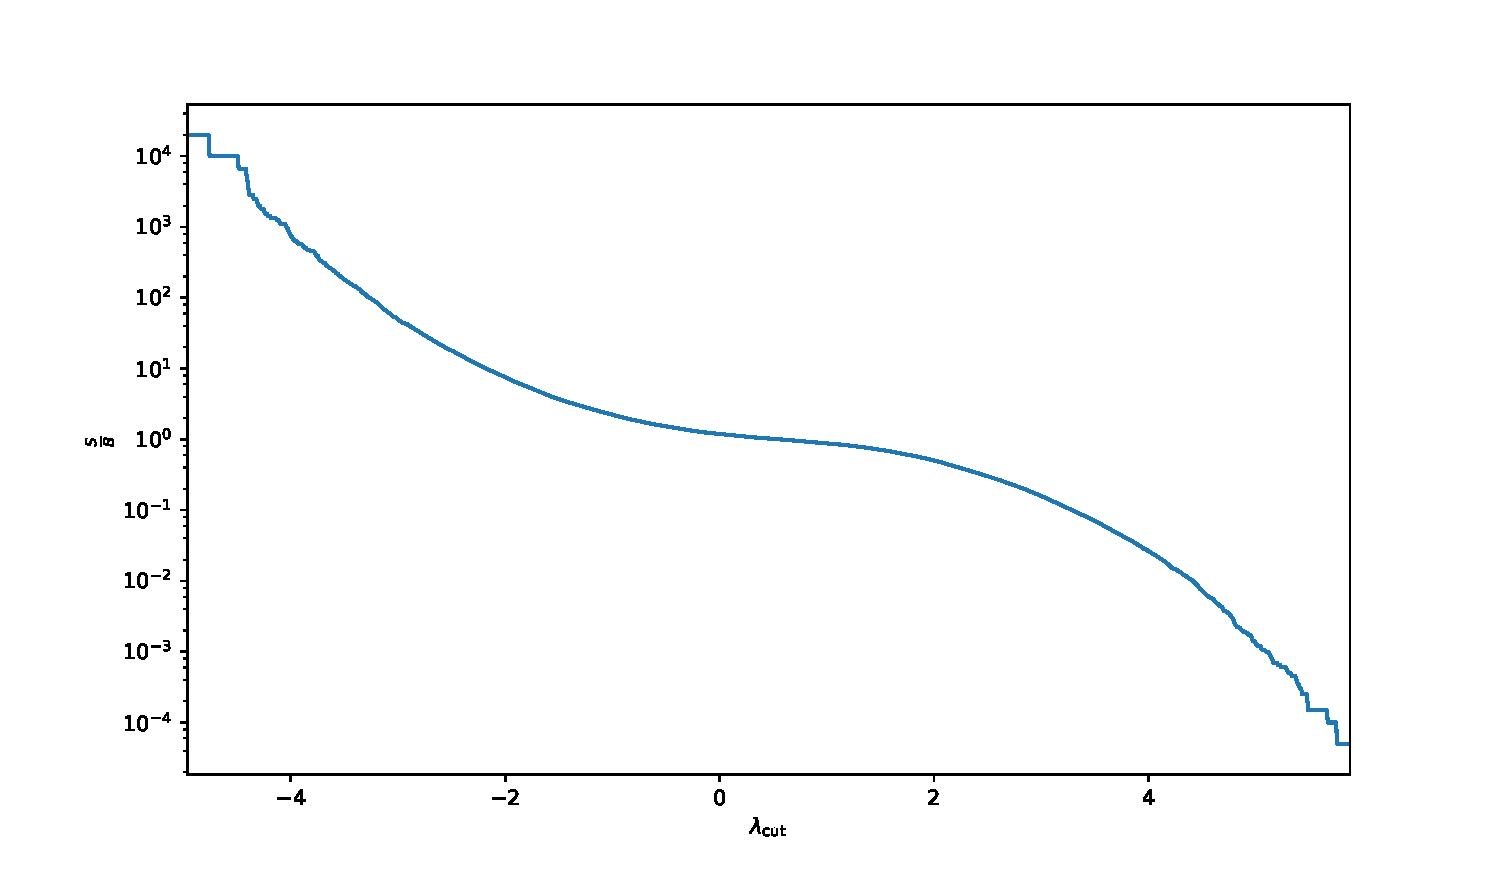
\includegraphics[width=\textwidth]{../A16/A16f_10000.pdf}
    \caption{Signal-zu-Untergrundverhältnis für $P_{0, 10000}$.}
    \label{fig:A16f_10000}
\end{figure}
\begin{figure}
    \centering
    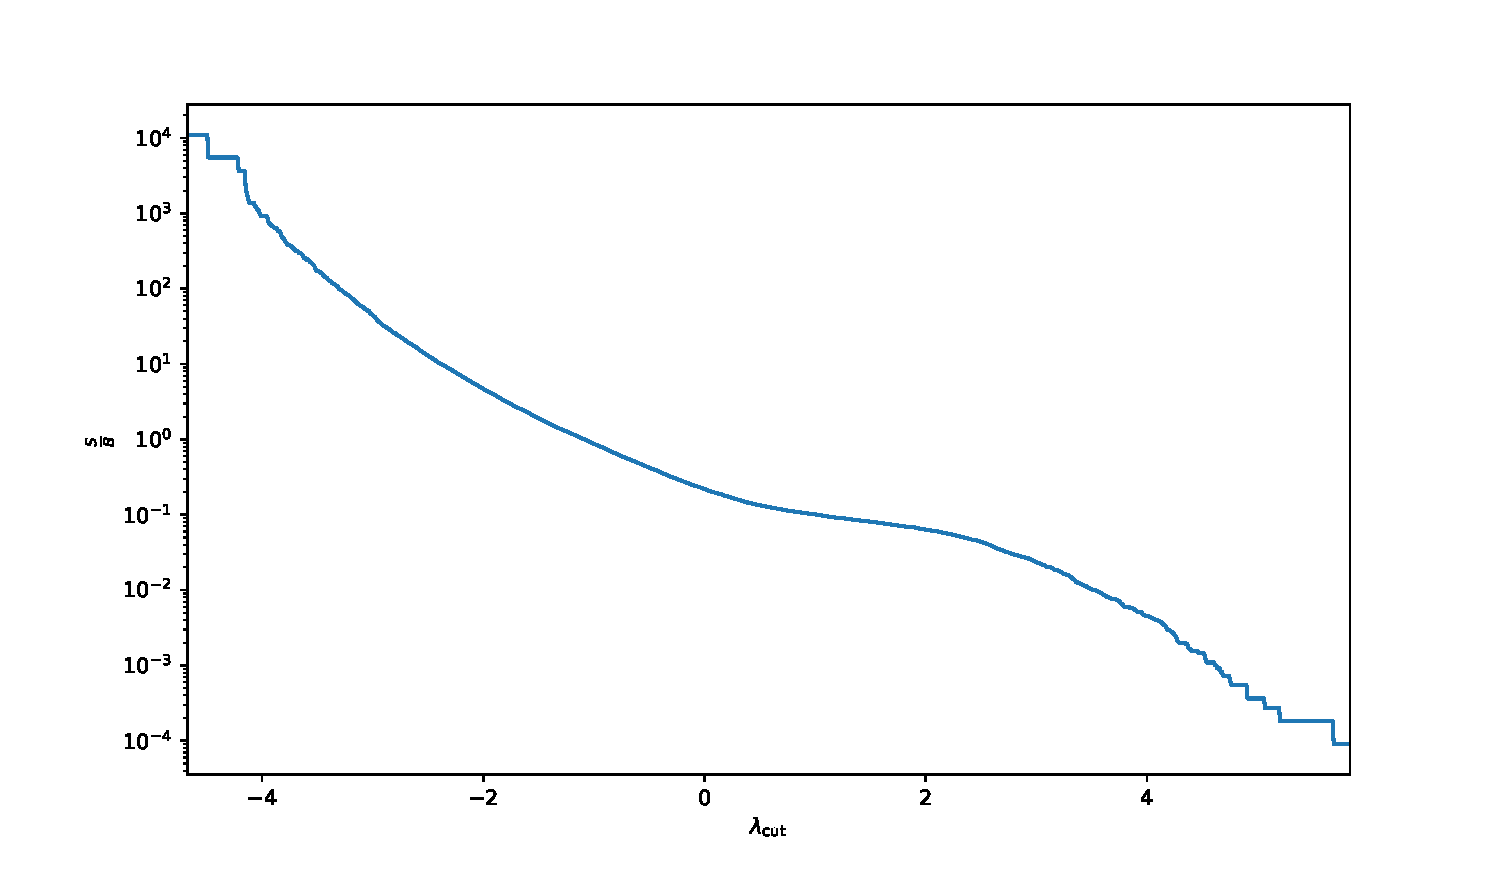
\includegraphics[width=\textwidth]{../A16/A16f_1000.pdf}
    \caption{Signal-zu-Untergrundverhältnis für $P_{0, 1000}$.}
    \label{fig:A16f_1000}
\end{figure}
\FloatBarrier

\subsection*{g)}
Die Signifikanz $\frac{S}{\sqrt{S + B}}$ wird maximal für $S + B \rightarrow 0$ also für $\lambda_\textup{cut} \rightarrow -\infty$.
\begin{figure}
    \centering
    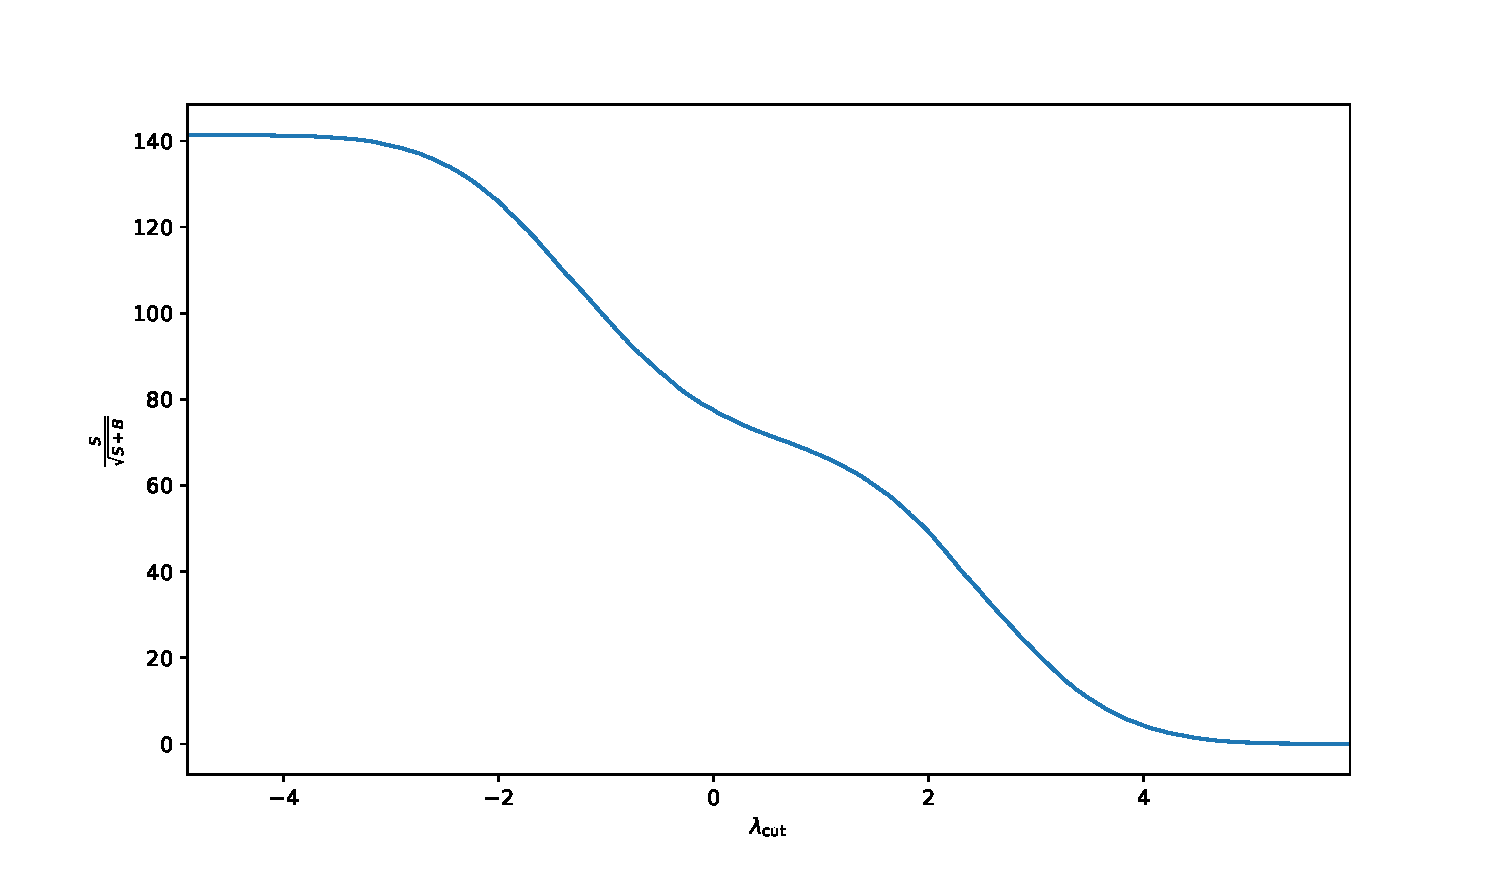
\includegraphics[width=\textwidth]{../A16/A16g_10000.pdf}
    \caption{Signifikanz für $P_{0, 10000}$.}
    \label{fig:A16g_10000}
\end{figure}
\begin{figure}
    \centering
    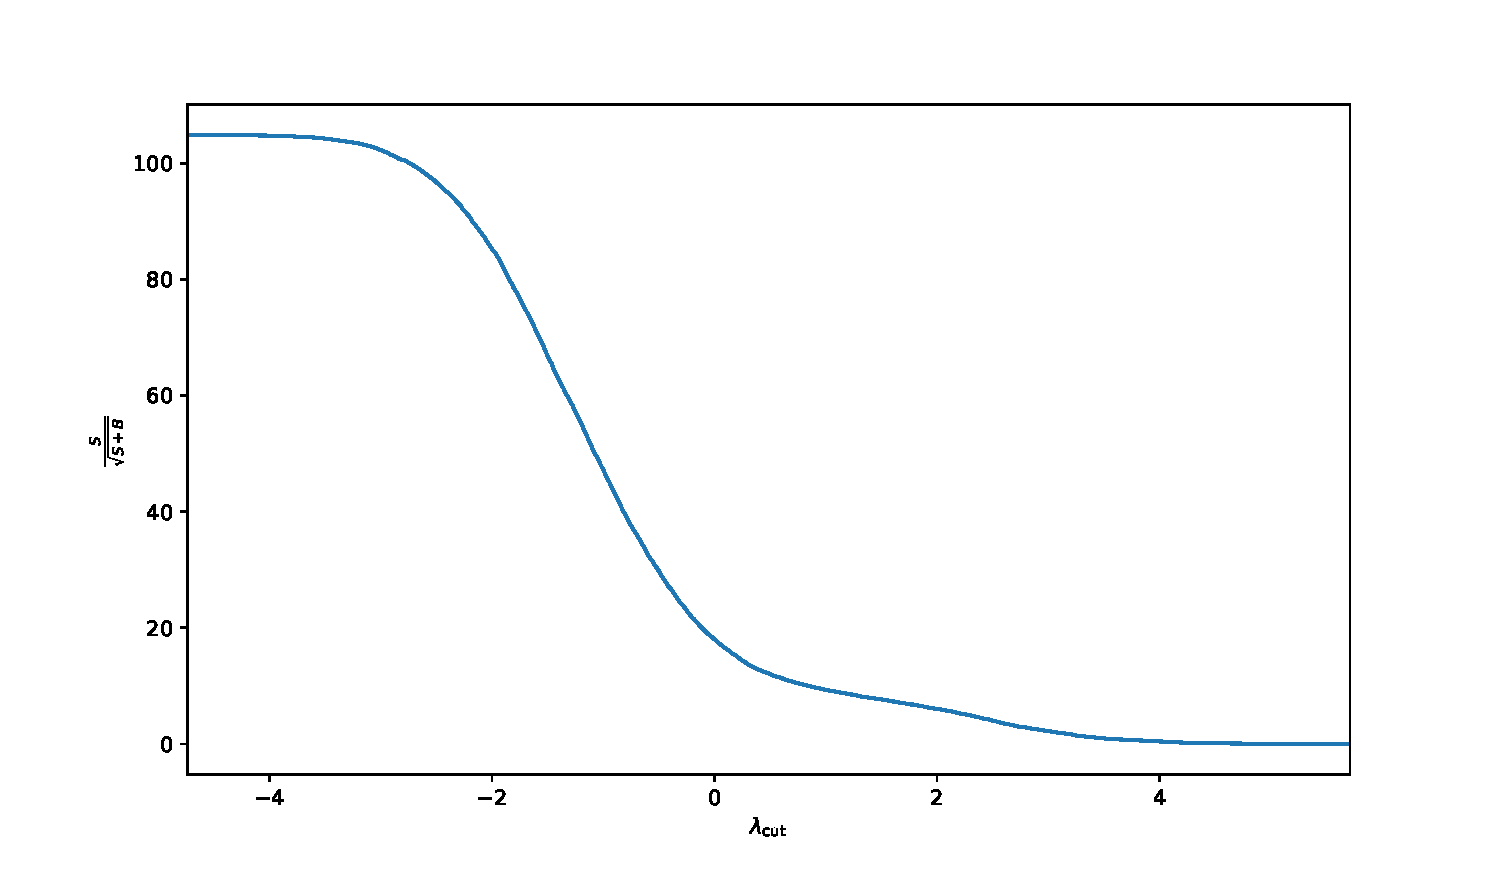
\includegraphics[width=\textwidth]{../A16/A16g_1000.pdf}
    \caption{Signifikanz für $P_{0, 1000}$.}
    \label{fig:A16g_1000}
\end{figure}
\FloatBarrier

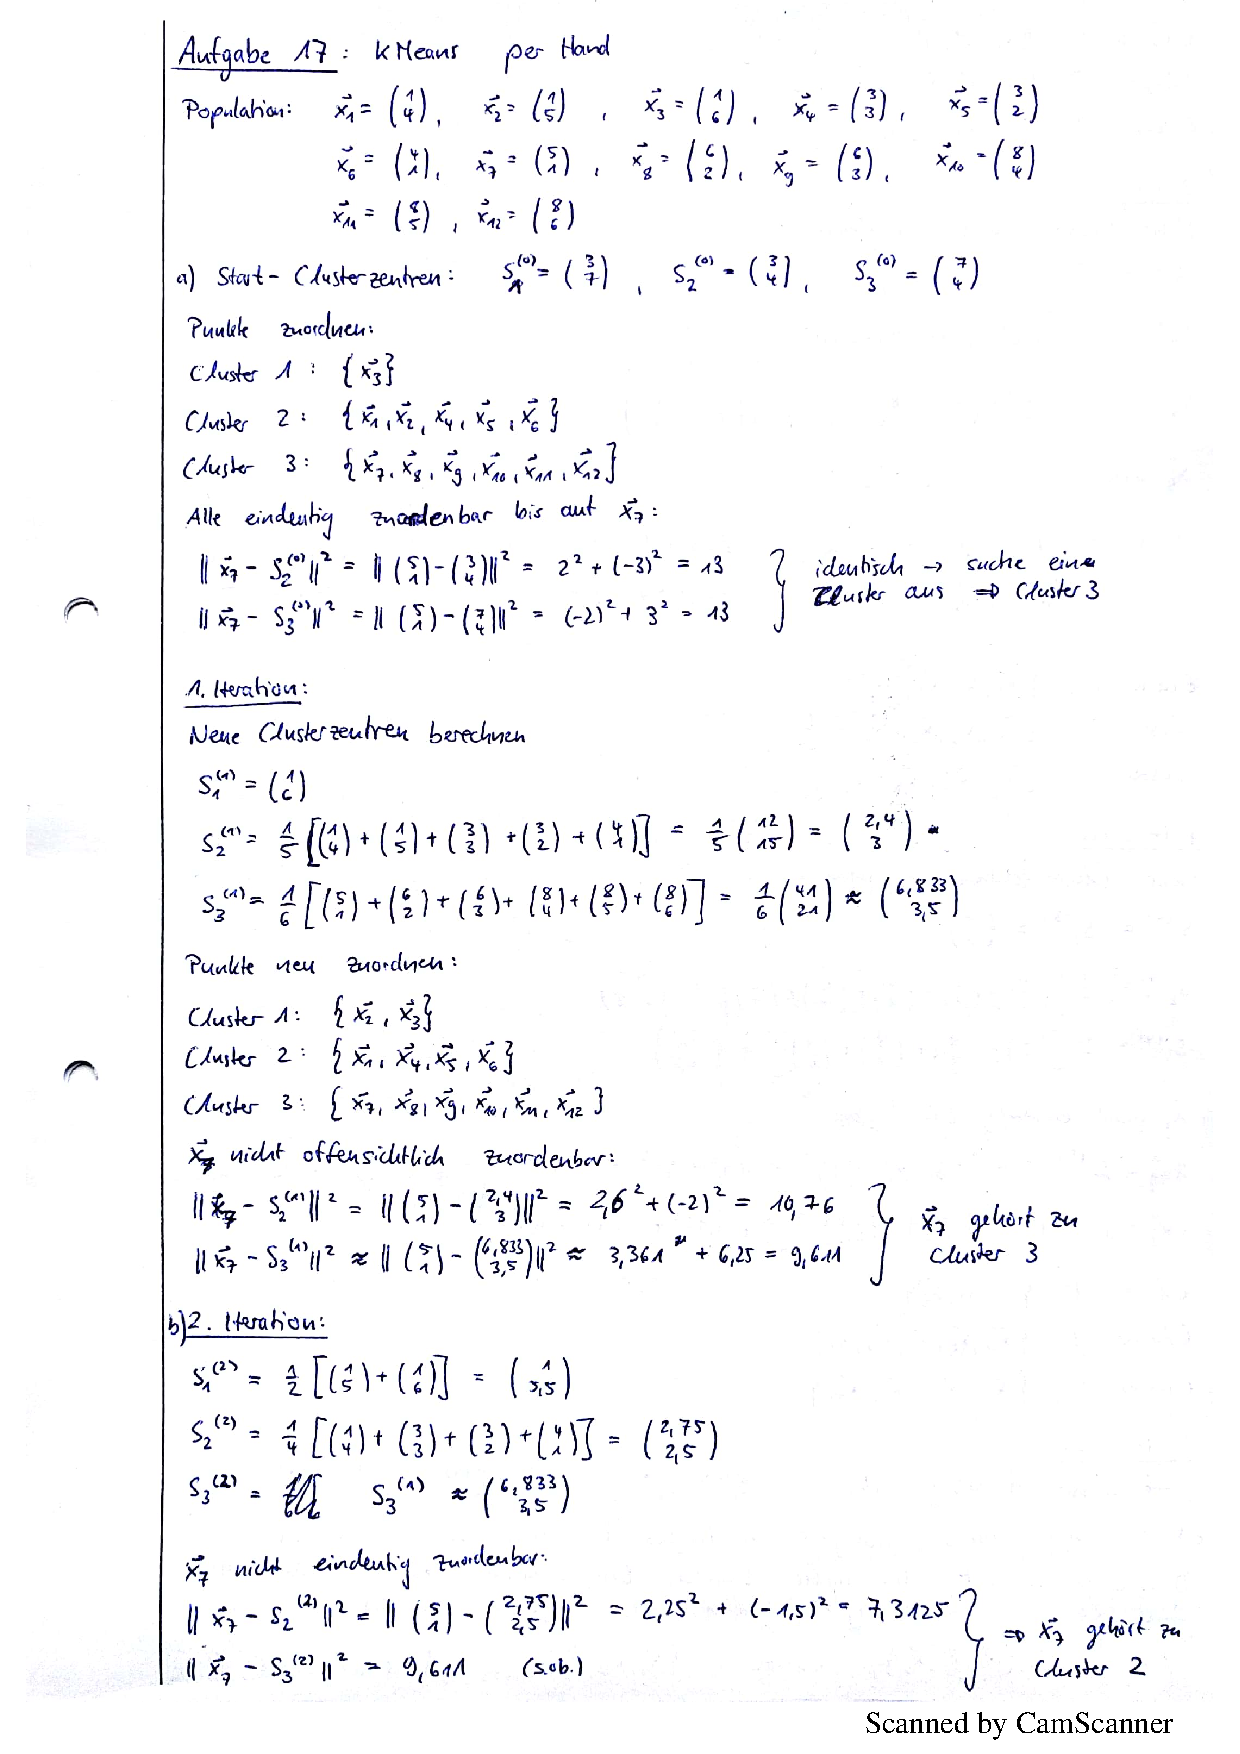
\includepdf[pages=-]{../SMD_B5_A17}

\section*{Aufgabe 18}
\subsection*{a)}
Die Blobs wurden in der Ebene der ersten beiden Dimensionen geplottet.
\begin{figure}
    \centering
    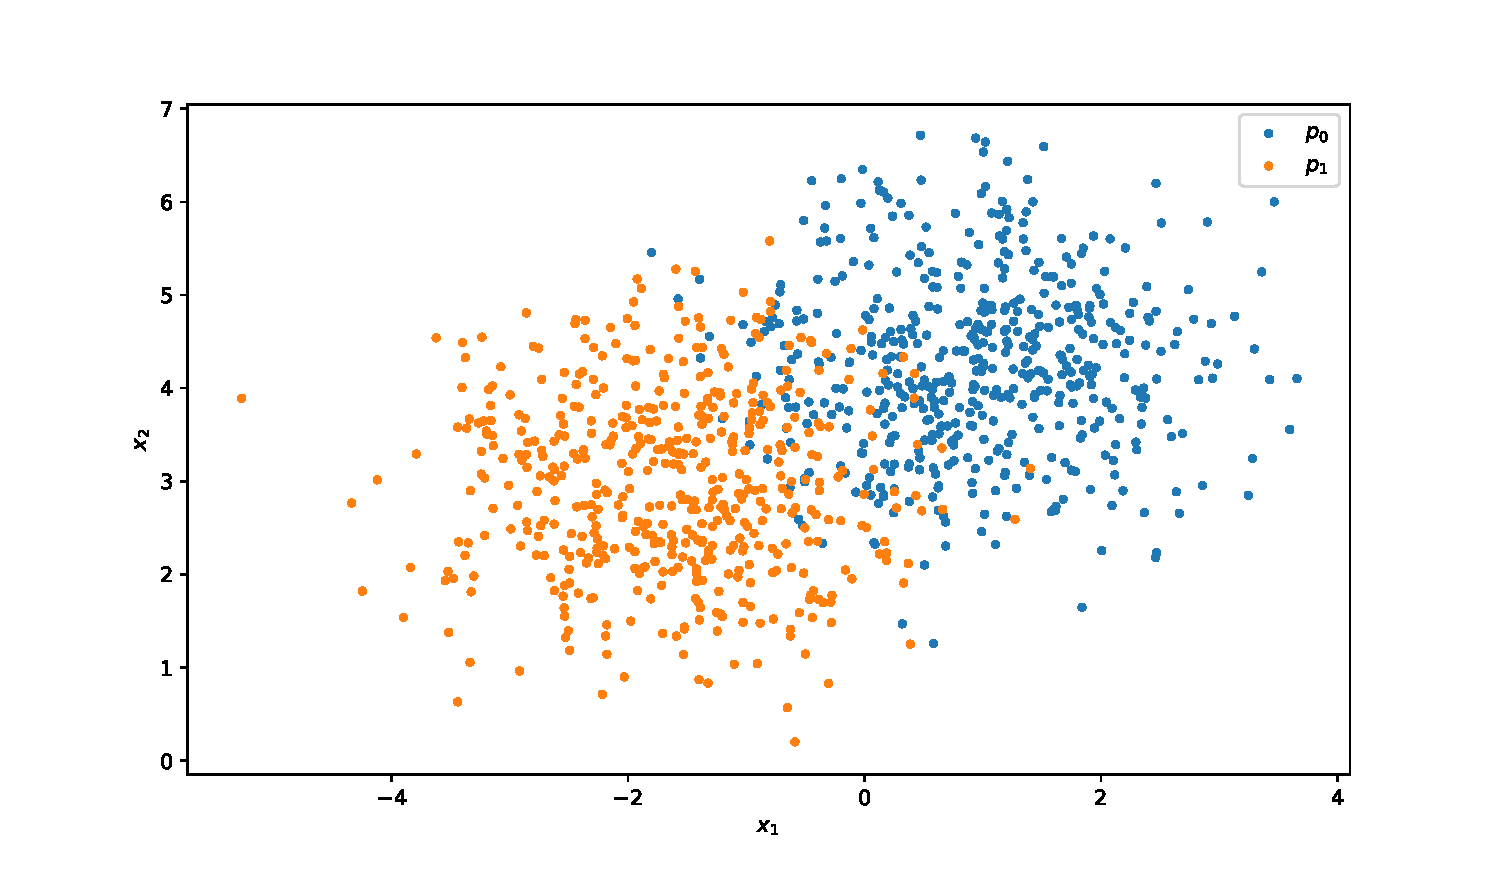
\includegraphics[width=\textwidth]{../A18/A18_scatter.pdf}
    \caption{Scatterplot in der Ebene der ersten beiden Dimension; untransformiert.}
    \label{fig:A18_scatter}
\end{figure}
\FloatBarrier

\subsection*{b)}
In der Hauptkomponentenanalyse sollen die Daten so transformiert werden, dass die Varianz entlang der Achsen extremal wird.
Das heißt, die Daten werden verschoben und vor allem gedreht, um am Ende einige Achsen zu haben, bei der die Daten möglichst weit auseinander liegen.
Sie haben also eine hohe Varianz.
Dadurch wird die Varianz entlang der anderen Achsen zwangsweise kleiner, die Populationen liegen also praktisch übereinander.
Diese Daten sind von keiner weiteren Bedeutung.

Der Ablauf:
\begin{enumerate}
    \item Zentrierung der Daten: Der Mittelwert aller Daten wird von den Daten abgezogen, damit sie danach vernünftig gedreht werden können.
    \item Berechnung der Kovarianzmatrix: Die Kovarianzmatrix wird benötigt, um eine Aussage über die Varianz treffen zu können.
    \item Berechnung der Eigenwerte und -vektoren: Mit den Eigenwerten kann die Kovarianzmatrix diagonalisiert werden.
    \item Die $k$ größten Eigenwerte und zugehörige Eigenvektoren werden ausgewählt: Da die Kovarianzmatrix mit den Eigenwerten diagonalisiert werden kann, kann mit den Eigenvektoren, die zu den größten Eigenwerten gehören, eine Transformationsmatrix aufgestellt werden, die die Varianz maximiert.
    \item Bildung eine $d\times k$ Matrix aus den $k$ Eigenvektoren: Dies ist die eben angesprochene Transformationsmatrix.
    \item Transformation der Daten mit der Transformationsmatrix: Auf diese Weise wird die Varianz der transformiert Daten $x'$ extremalisiert.
\end{enumerate}

\subsection*{c)}
Die Eigenwerte lauten:
\begin{align*}
    \lambda_1 &\approx 17,5 \\
    \lambda_2 &\approx 0,999\\
    \lambda_3 &\approx 0,987\\
    \lambda_4 &\approx 0,898
\end{align*}
Daran wird direkt erkennlich, dass die Daten entlang der ersten Achse sehr gut getrennt werden und entlang der anderen Achsen sehr schlecht.

\subsection*{d)}
\begin{figure}
    \centering
    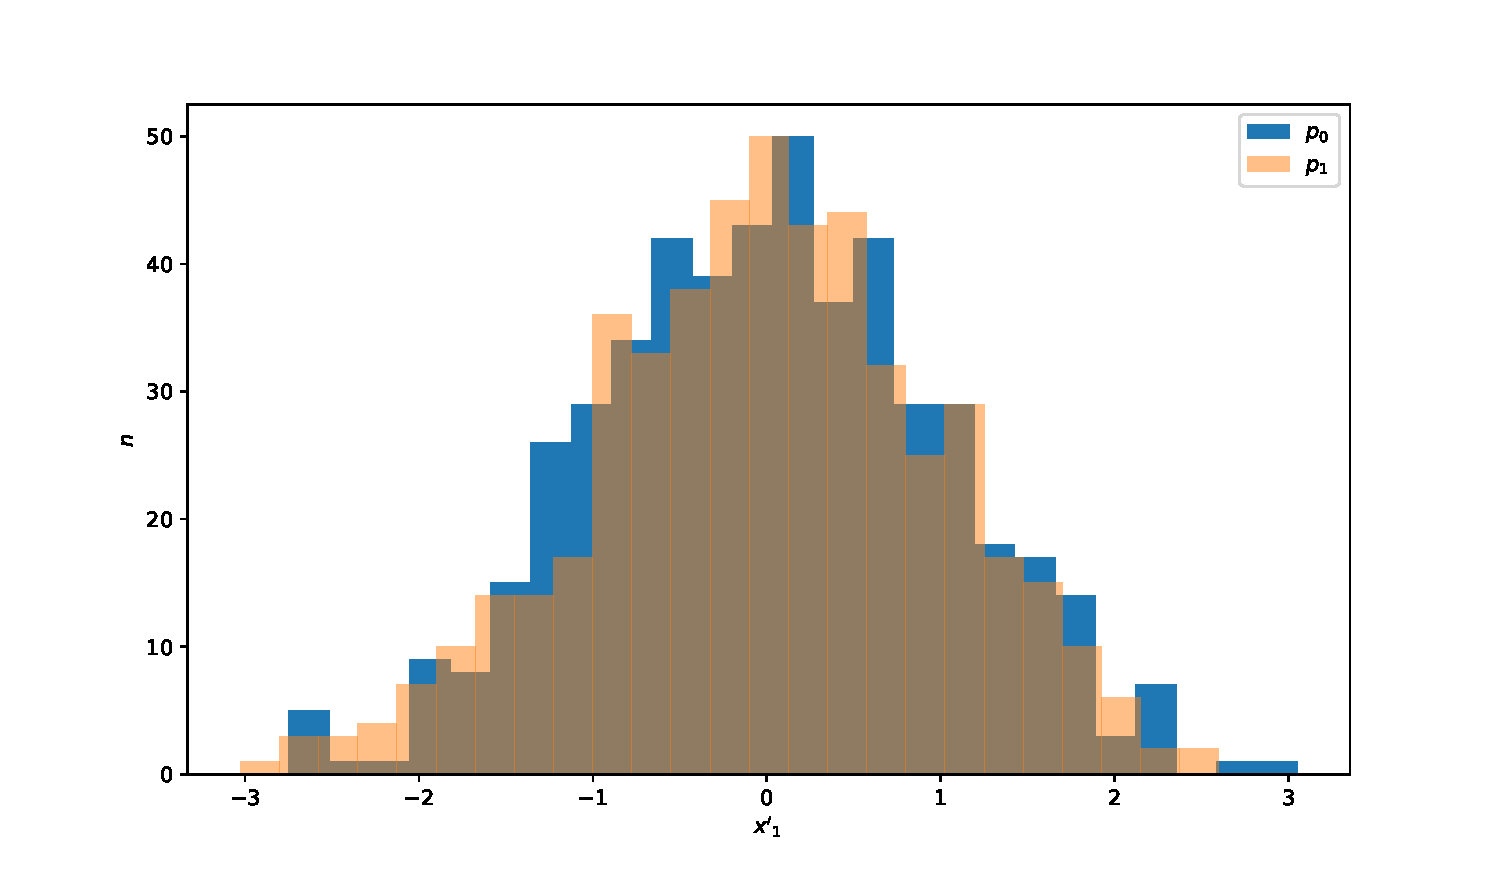
\includegraphics[width=\textwidth]{../A18/A18_hist_1.pdf}
    \caption{Histogramm für die Projektion auf die erste Achse.}
    \label{fig:A18_hist_1}
\end{figure}
\begin{figure}
    \centering
    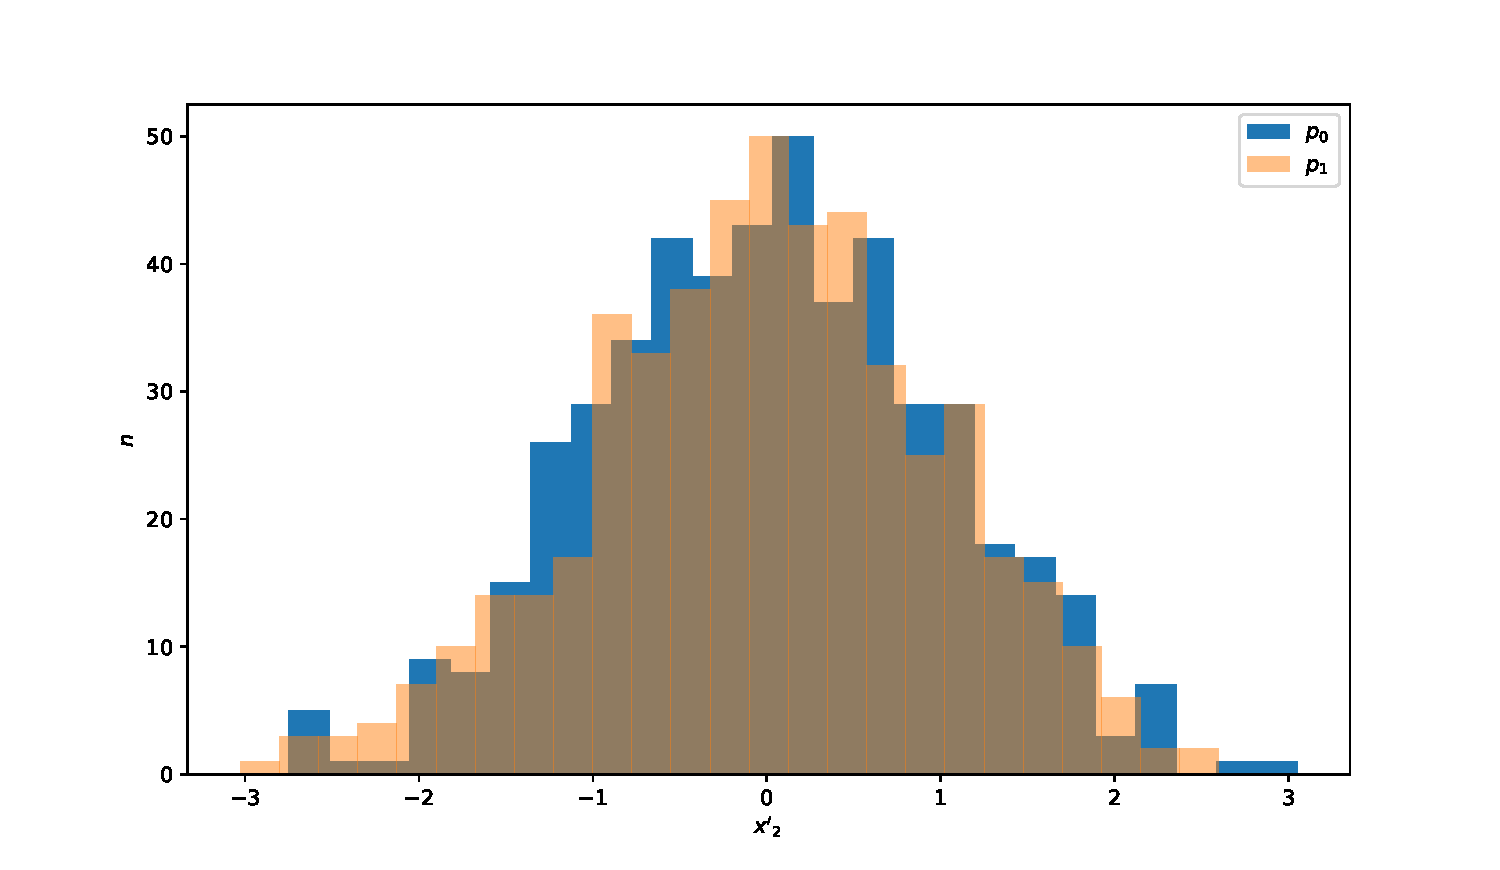
\includegraphics[width=\textwidth]{../A18/A18_hist_2.pdf}
    \caption{Histogramm für die Projektion auf die zweiten Achse.}
    \label{fig:A18_hist_2}
\end{figure}
\begin{figure}
    \centering
    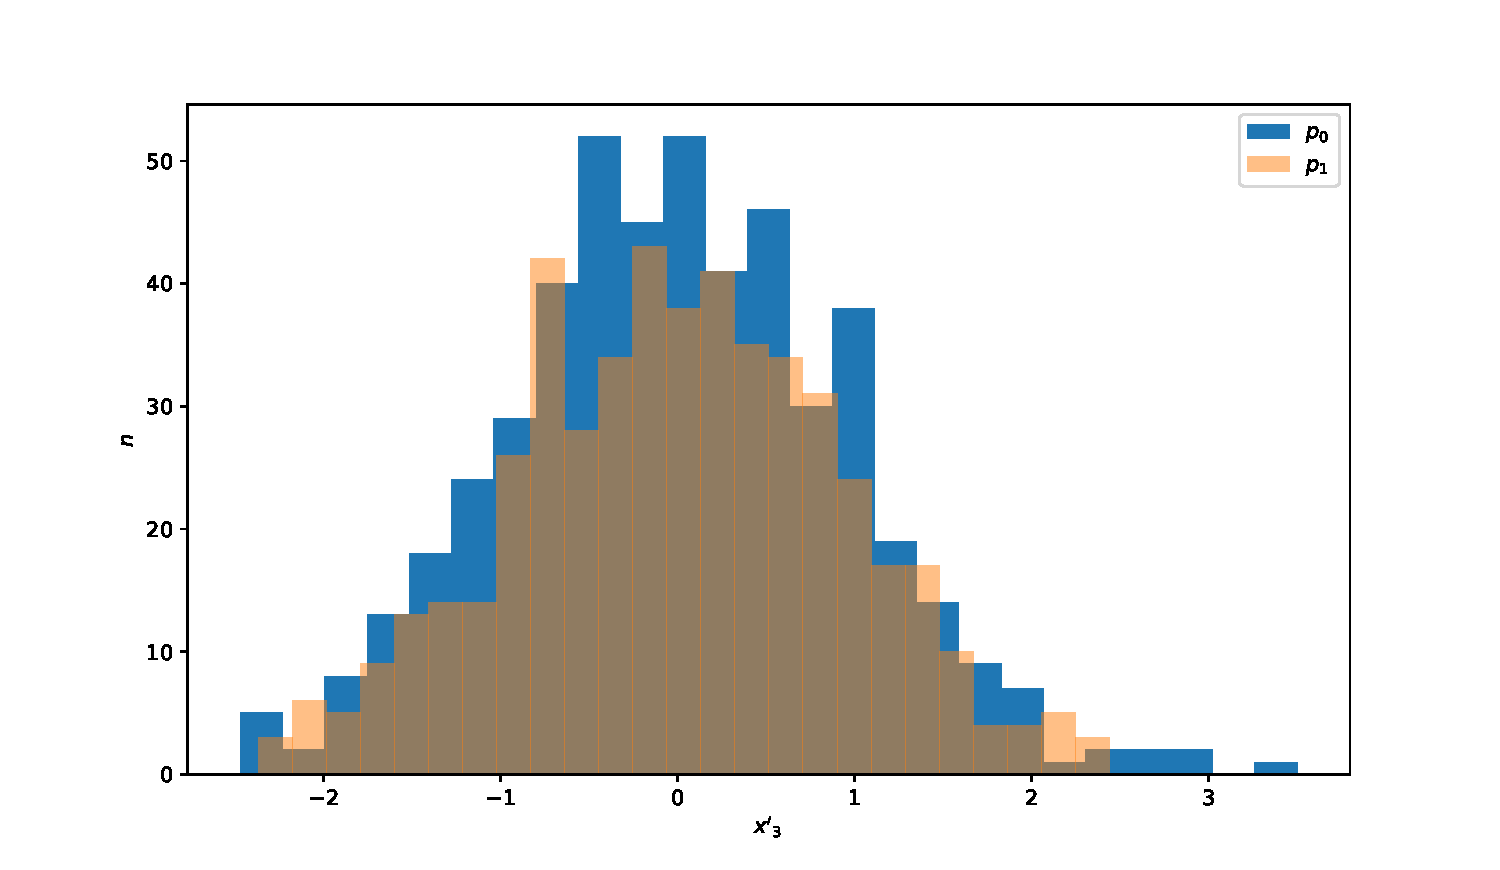
\includegraphics[width=\textwidth]{../A18/A18_hist_3.pdf}
    \caption{Histogramm für die Projektion auf die dritten Achse.}
    \label{fig:A18_hist_3}
\end{figure}
\begin{figure}
    \centering
    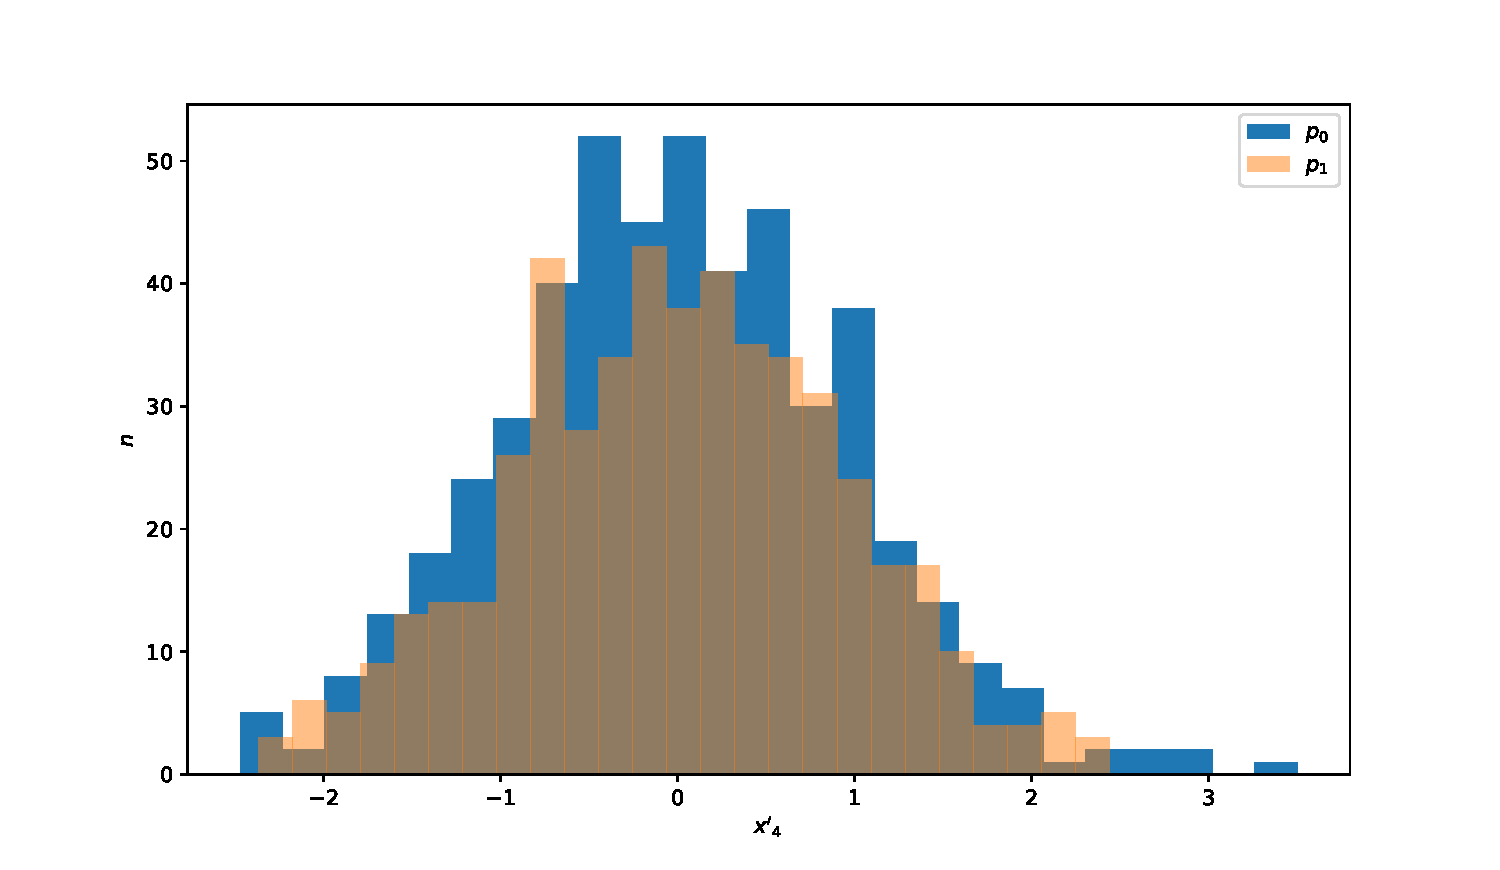
\includegraphics[width=\textwidth]{../A18/A18_hist_4.pdf}
    \caption{Histogramm für die Projektion auf die vierten Achse.}
    \label{fig:A18_hist_4}
\end{figure}
\begin{figure}
    \centering
    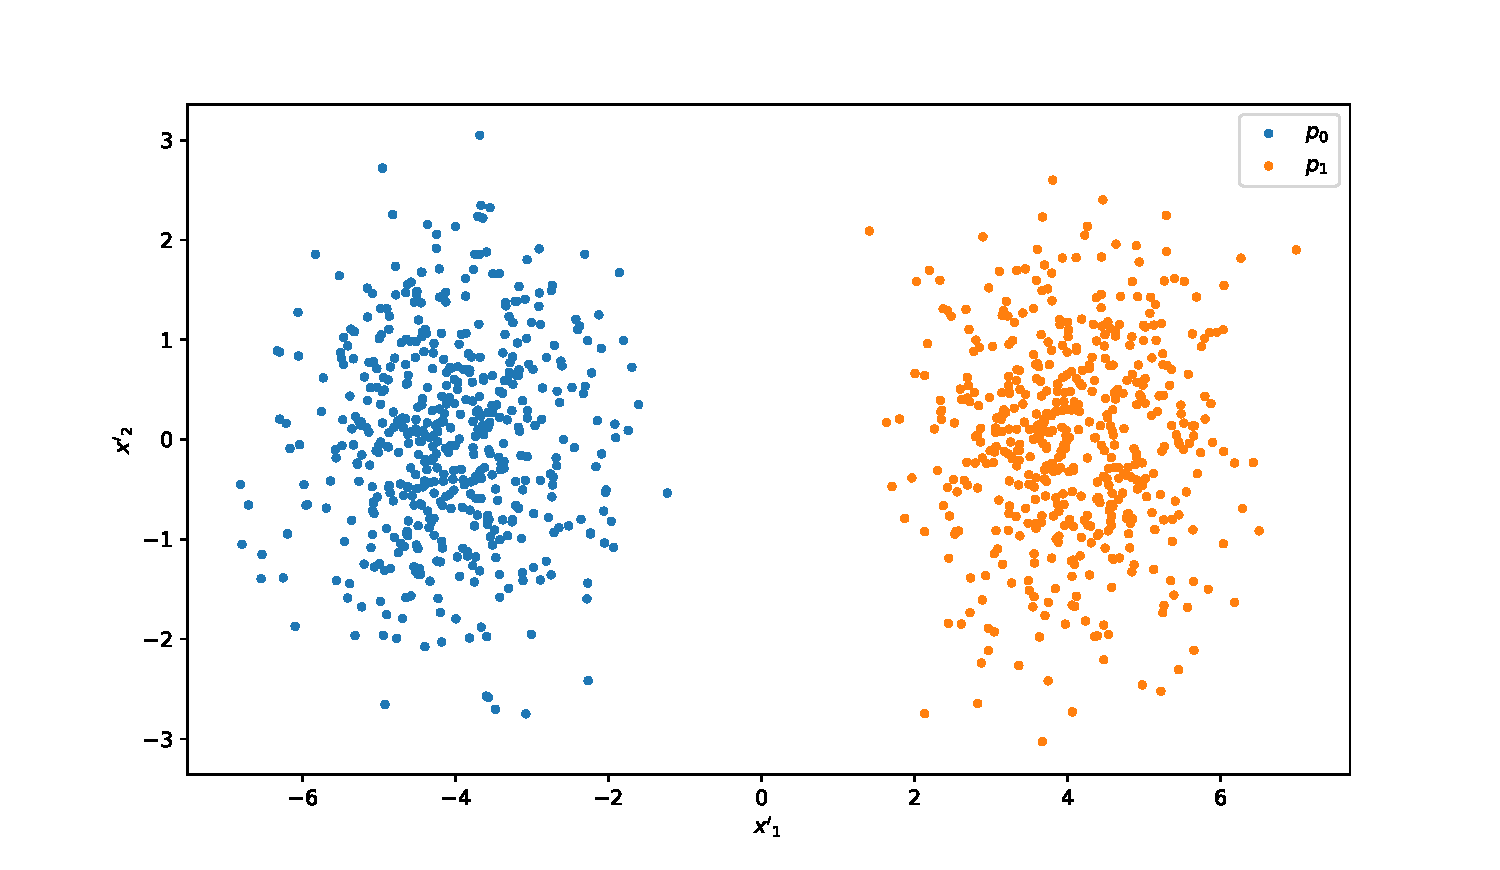
\includegraphics[width=\textwidth]{../A18/A18_transformed_scatter.pdf}
    \caption{Scatterplot in der Ebene der ersten beiden transformierten Dimensionen.}
    \label{fig:A18_transformed_scatter}
\end{figure}
\FloatBarrier
Anhand der Histogramme ist deutlich ersichtlich, dass die Daten lediglich in der ersten transformierten Dimension gut trennbar sind.
Die Erwartung, die aus den Eigenwerten folgte, wurde damit bestätigt.
Dies ist auch an dem Scatterplot \ref{fig:A18_transformed_scatter} ersichtlich, da die Daten zwar sehr deutlich nach links und rechts, also entlang der $x'_1$ Dimension, trennbar sind, allerdings nicht nach oben und unten, also entlang der $x'_2$ Dimension, trennbar sind.


\end{document}
